% Options for packages loaded elsewhere
\PassOptionsToPackage{unicode}{hyperref}
\PassOptionsToPackage{hyphens}{url}
%
\documentclass[
  ignorenonframetext,
]{beamer}
\usepackage{pgfpages}
\setbeamertemplate{caption}[numbered]
\setbeamertemplate{caption label separator}{: }
\setbeamercolor{caption name}{fg=normal text.fg}
\beamertemplatenavigationsymbolsempty
% Prevent slide breaks in the middle of a paragraph
\widowpenalties 1 10000
\raggedbottom
\setbeamertemplate{part page}{
  \centering
  \begin{beamercolorbox}[sep=16pt,center]{part title}
    \usebeamerfont{part title}\insertpart\par
  \end{beamercolorbox}
}
\setbeamertemplate{section page}{
  \centering
  \begin{beamercolorbox}[sep=12pt,center]{part title}
    \usebeamerfont{section title}\insertsection\par
  \end{beamercolorbox}
}
\setbeamertemplate{subsection page}{
  \centering
  \begin{beamercolorbox}[sep=8pt,center]{part title}
    \usebeamerfont{subsection title}\insertsubsection\par
  \end{beamercolorbox}
}
\AtBeginPart{
  \frame{\partpage}
}
\AtBeginSection{
  \ifbibliography
  \else
    \frame{\sectionpage}
  \fi
}
\AtBeginSubsection{
  \frame{\subsectionpage}
}

\usepackage{amsmath,amssymb}
\usepackage{lmodern}
\usepackage{iftex}
\ifPDFTeX
  \usepackage[T1]{fontenc}
  \usepackage[utf8]{inputenc}
  \usepackage{textcomp} % provide euro and other symbols
\else % if luatex or xetex
  \usepackage{unicode-math}
  \defaultfontfeatures{Scale=MatchLowercase}
  \defaultfontfeatures[\rmfamily]{Ligatures=TeX,Scale=1}
  \setmainfont[]{VisbyCF-Medium}
  \setsansfont[]{Latin Modern Sans}
  \setmathfont[]{Latin Modern Math}
\fi
\usecolortheme{Flip}
\usefonttheme{serif} % use mainfont rather than sansfont for slide text
\useinnertheme{Flip}
\useoutertheme{Flip}
% Use upquote if available, for straight quotes in verbatim environments
\IfFileExists{upquote.sty}{\usepackage{upquote}}{}
\IfFileExists{microtype.sty}{% use microtype if available
  \usepackage[]{microtype}
  \UseMicrotypeSet[protrusion]{basicmath} % disable protrusion for tt fonts
}{}
\makeatletter
\@ifundefined{KOMAClassName}{% if non-KOMA class
  \IfFileExists{parskip.sty}{%
    \usepackage{parskip}
  }{% else
    \setlength{\parindent}{0pt}
    \setlength{\parskip}{6pt plus 2pt minus 1pt}}
}{% if KOMA class
  \KOMAoptions{parskip=half}}
\makeatother
\usepackage{xcolor}
\newif\ifbibliography
\setlength{\emergencystretch}{3em} % prevent overfull lines
\setcounter{secnumdepth}{-\maxdimen} % remove section numbering

\usepackage{color}
\usepackage{fancyvrb}
\newcommand{\VerbBar}{|}
\newcommand{\VERB}{\Verb[commandchars=\\\{\}]}
\DefineVerbatimEnvironment{Highlighting}{Verbatim}{commandchars=\\\{\}}
% Add ',fontsize=\small' for more characters per line
\usepackage{framed}
\definecolor{shadecolor}{RGB}{241,243,245}
\newenvironment{Shaded}{\begin{snugshade}}{\end{snugshade}}
\newcommand{\AlertTok}[1]{\textcolor[rgb]{0.68,0.00,0.00}{#1}}
\newcommand{\AnnotationTok}[1]{\textcolor[rgb]{0.37,0.37,0.37}{#1}}
\newcommand{\AttributeTok}[1]{\textcolor[rgb]{0.40,0.45,0.13}{#1}}
\newcommand{\BaseNTok}[1]{\textcolor[rgb]{0.68,0.00,0.00}{#1}}
\newcommand{\BuiltInTok}[1]{\textcolor[rgb]{0.00,0.23,0.31}{#1}}
\newcommand{\CharTok}[1]{\textcolor[rgb]{0.13,0.47,0.30}{#1}}
\newcommand{\CommentTok}[1]{\textcolor[rgb]{0.37,0.37,0.37}{#1}}
\newcommand{\CommentVarTok}[1]{\textcolor[rgb]{0.37,0.37,0.37}{\textit{#1}}}
\newcommand{\ConstantTok}[1]{\textcolor[rgb]{0.56,0.35,0.01}{#1}}
\newcommand{\ControlFlowTok}[1]{\textcolor[rgb]{0.00,0.23,0.31}{#1}}
\newcommand{\DataTypeTok}[1]{\textcolor[rgb]{0.68,0.00,0.00}{#1}}
\newcommand{\DecValTok}[1]{\textcolor[rgb]{0.68,0.00,0.00}{#1}}
\newcommand{\DocumentationTok}[1]{\textcolor[rgb]{0.37,0.37,0.37}{\textit{#1}}}
\newcommand{\ErrorTok}[1]{\textcolor[rgb]{0.68,0.00,0.00}{#1}}
\newcommand{\ExtensionTok}[1]{\textcolor[rgb]{0.00,0.23,0.31}{#1}}
\newcommand{\FloatTok}[1]{\textcolor[rgb]{0.68,0.00,0.00}{#1}}
\newcommand{\FunctionTok}[1]{\textcolor[rgb]{0.28,0.35,0.67}{#1}}
\newcommand{\ImportTok}[1]{\textcolor[rgb]{0.00,0.46,0.62}{#1}}
\newcommand{\InformationTok}[1]{\textcolor[rgb]{0.37,0.37,0.37}{#1}}
\newcommand{\KeywordTok}[1]{\textcolor[rgb]{0.00,0.23,0.31}{#1}}
\newcommand{\NormalTok}[1]{\textcolor[rgb]{0.00,0.23,0.31}{#1}}
\newcommand{\OperatorTok}[1]{\textcolor[rgb]{0.37,0.37,0.37}{#1}}
\newcommand{\OtherTok}[1]{\textcolor[rgb]{0.00,0.23,0.31}{#1}}
\newcommand{\PreprocessorTok}[1]{\textcolor[rgb]{0.68,0.00,0.00}{#1}}
\newcommand{\RegionMarkerTok}[1]{\textcolor[rgb]{0.00,0.23,0.31}{#1}}
\newcommand{\SpecialCharTok}[1]{\textcolor[rgb]{0.37,0.37,0.37}{#1}}
\newcommand{\SpecialStringTok}[1]{\textcolor[rgb]{0.13,0.47,0.30}{#1}}
\newcommand{\StringTok}[1]{\textcolor[rgb]{0.13,0.47,0.30}{#1}}
\newcommand{\VariableTok}[1]{\textcolor[rgb]{0.07,0.07,0.07}{#1}}
\newcommand{\VerbatimStringTok}[1]{\textcolor[rgb]{0.13,0.47,0.30}{#1}}
\newcommand{\WarningTok}[1]{\textcolor[rgb]{0.37,0.37,0.37}{\textit{#1}}}

\providecommand{\tightlist}{%
  \setlength{\itemsep}{0pt}\setlength{\parskip}{0pt}}\usepackage{longtable,booktabs,array}
\usepackage{calc} % for calculating minipage widths
\usepackage{caption}
% Make caption package work with longtable
\makeatletter
\def\fnum@table{\tablename~\thetable}
\makeatother
\usepackage{graphicx}
\makeatletter
\def\maxwidth{\ifdim\Gin@nat@width>\linewidth\linewidth\else\Gin@nat@width\fi}
\def\maxheight{\ifdim\Gin@nat@height>\textheight\textheight\else\Gin@nat@height\fi}
\makeatother
% Scale images if necessary, so that they will not overflow the page
% margins by default, and it is still possible to overwrite the defaults
% using explicit options in \includegraphics[width, height, ...]{}
\setkeys{Gin}{width=\maxwidth,height=\maxheight,keepaspectratio}
% Set default figure placement to htbp
\makeatletter
\def\fps@figure{htbp}
\makeatother

\usepackage{booktabs}
\usepackage{longtable}
\usepackage{array}
\usepackage{multirow}
\usepackage{wrapfig}
\usepackage{float}
\usepackage{colortbl}
\usepackage{pdflscape}
\usepackage{tabu}
\usepackage{threeparttable}
\usepackage{threeparttablex}
\usepackage[normalem]{ulem}
\usepackage{makecell}
\usepackage{xcolor}
\usepackage{tabu}
\usepackage{mathtools}
\usepackage{mathrsfs}
\makeatletter
\makeatother
\makeatletter
\makeatother
\makeatletter
\@ifpackageloaded{caption}{}{\usepackage{caption}}
\AtBeginDocument{%
\ifdefined\contentsname
  \renewcommand*\contentsname{Table of contents}
\else
  \newcommand\contentsname{Table of contents}
\fi
\ifdefined\listfigurename
  \renewcommand*\listfigurename{List of Figures}
\else
  \newcommand\listfigurename{List of Figures}
\fi
\ifdefined\listtablename
  \renewcommand*\listtablename{List of Tables}
\else
  \newcommand\listtablename{List of Tables}
\fi
\ifdefined\figurename
  \renewcommand*\figurename{Figure}
\else
  \newcommand\figurename{Figure}
\fi
\ifdefined\tablename
  \renewcommand*\tablename{Table}
\else
  \newcommand\tablename{Table}
\fi
}
\@ifpackageloaded{float}{}{\usepackage{float}}
\floatstyle{ruled}
\@ifundefined{c@chapter}{\newfloat{codelisting}{h}{lop}}{\newfloat{codelisting}{h}{lop}[chapter]}
\floatname{codelisting}{Listing}
\newcommand*\listoflistings{\listof{codelisting}{List of Listings}}
\makeatother
\makeatletter
\@ifpackageloaded{caption}{}{\usepackage{caption}}
\@ifpackageloaded{subcaption}{}{\usepackage{subcaption}}
\makeatother
\makeatletter
\@ifpackageloaded{tcolorbox}{}{\usepackage[many]{tcolorbox}}
\makeatother
\makeatletter
\@ifundefined{shadecolor}{\definecolor{shadecolor}{rgb}{.97, .97, .97}}
\makeatother
\makeatletter
\makeatother
\ifLuaTeX
  \usepackage{selnolig}  % disable illegal ligatures
\fi
\IfFileExists{bookmark.sty}{\usepackage{bookmark}}{\usepackage{hyperref}}
\IfFileExists{xurl.sty}{\usepackage{xurl}}{} % add URL line breaks if available
\urlstyle{same} % disable monospaced font for URLs
\hypersetup{
  pdftitle={Analyse de survie},
  pdfauthor={Léo Belzile},
  hidelinks,
  pdfcreator={LaTeX via pandoc}}

\title{Analyse de survie}
\subtitle{Analyse multidimensionnelle appliquée}
\author{Léo Belzile}
\date{}
\institute{HEC Montréal}

\begin{document}
\frame{\titlepage}
\ifdefined\Shaded\renewenvironment{Shaded}{\begin{tcolorbox}[interior hidden, frame hidden, borderline west={3pt}{0pt}{shadecolor}, enhanced, breakable, sharp corners, boxrule=0pt]}{\end{tcolorbox}}\fi

\begin{frame}{Modèle à risques proportionnels de Cox}
\protect\hypertarget{moduxe8le-uxe0-risques-proportionnels-de-cox}{}
Le \textbf{modèle à risques proportionnels de Cox} pour \(\mathbf{X}\)
au temps \(t\) est \begin{align*}
h(t; \mathbf{X}) = h_0(t)\exp(\beta_1\mathrm{X}_1 + \cdots + \beta_p \mathrm{X}_p),
\end{align*} où \(h_0(t)\) est la fonction de risque de base qui
remplace l'ordonnée à l'origine.

\begin{itemize}
\tightlist
\item
  Postulat de risques proportionnels: le rapport de risque pour deux
  observations ne varie pas en fonction du temps \(t\).
\end{itemize}
\end{frame}

\begin{frame}{Postulat de risques proportionnels}
\protect\hypertarget{postulat-de-risques-proportionnels}{}
\begin{figure}

{\centering \includegraphics[width=0.9\textwidth,height=\textheight]{MATH60602-diapos9_files/figure-beamer/fig-risquepropfig-1.pdf}

}

\caption{\label{fig-risquepropfig}Courbes de risques proportionnelles
(panneau supérieur) et non proportionnelles (panneau inférieur).}

\end{figure}
\end{frame}

\begin{frame}{Absence de proportionnalité et stratification}
\protect\hypertarget{absence-de-proportionnalituxe9-et-stratification}{}
On peut modéliser la non proportionnalité des risques par la
\textbf{stratification} pour une variable catégorielle
\(Z=1, \ldots, K\).

Supposons que l'effet de \(Z\) sur le risque varie dans le temps.

On écrit alors \begin{align*}
h(t; \mathbf{X}, Z=k) = h_k(t)\exp(\beta_1\mathrm{X}_1 + \cdots + \beta_p \mathrm{X}_p),
\end{align*} où \(h_k(t)\) est la fonction de risque de base pour
\(Z=k\).

Dans ce modèle

\begin{itemize}
\tightlist
\item
  On suppose que l'effet des variables explicatives \(\mathbf{X}\) est
  le même peut importe la valeur de \(Z\).
\item
  L'effet de \(Z=k\) vs \(Z=j\) pour un même ensemble de variables
  explicatives \(\mathbf{X}\) est \(h_k(t)/h_j(t)\), qui dépend du
  temps.
\end{itemize}
\end{frame}

\begin{frame}{Stratification}
\protect\hypertarget{stratification}{}
\begin{itemize}
\tightlist
\item
  \textbf{Avantage}: on peut modéliser n'importe quel changement du
  risque en fonction de \(Z\).
\item
  \textbf{Désavantage}: on perd la variable explicative \(Z\), donc on
  ne peut tester son effet (pas de coefficient)\ldots{} on peut résumer
  l'information pour la variable \(Z\) en calculant par exemple les
  différences de survie à des temps donnés.
\item
  \textbf{Désavantage}: la fonction de risque est estimée pour chaque
  sous-groupe de \(Z\) (plus faible taille d'échantillon).
\end{itemize}

Idéalement, utiliser la stratification avec des variables secondaires ou
de contrôles.
\end{frame}

\begin{frame}[fragile]{Modèle de Cox avec stratification dans
\textbf{R}}
\protect\hypertarget{moduxe8le-de-cox-avec-stratification-dans-r}{}
\begin{Shaded}
\begin{Highlighting}[numbers=left,,]
\FunctionTok{library}\NormalTok{(survival)}
\FunctionTok{data}\NormalTok{(survie1, }\AttributeTok{package =} \StringTok{"hecmulti"}\NormalTok{)}
\CommentTok{\# Stratification par service}
\NormalTok{cox\_strat }\OtherTok{\textless{}{-}} \FunctionTok{coxph}\NormalTok{(}
  \FunctionTok{Surv}\NormalTok{(temps, censure) }\SpecialCharTok{\textasciitilde{}}\NormalTok{ age }\SpecialCharTok{+}\NormalTok{ sexe }\SpecialCharTok{+} \FunctionTok{strata}\NormalTok{(service), }
  \AttributeTok{data =}\NormalTok{ survie1)}
\CommentTok{\# Décompte par service}
\FunctionTok{with}\NormalTok{(survie1, }\FunctionTok{table}\NormalTok{(censure, service))}
\CommentTok{\# Coefficients}
\FunctionTok{summary}\NormalTok{(cox\_strat)}
\end{Highlighting}
\end{Shaded}
\end{frame}

\begin{frame}{Sorties}
\protect\hypertarget{sorties}{}
\hypertarget{tbl-nserv}{}
\begin{table}
\caption{\label{tbl-nserv}Décompte du nombre d'observations par service et status. }\tabularnewline

\centering
\begin{tabular}{lrrrr}
\toprule
  & 0 & 1 & 2 & 3\\
\midrule
0 & 37 & 66 & 37 & 26\\
1 & 160 & 113 & 41 & 20\\
\bottomrule
\end{tabular}
\end{table}

\hypertarget{tbl-coxstratif}{}
\begin{table}
\caption{\label{tbl-coxstratif}Rapport de risques pour un modèle de Cox stratifié par service. }\tabularnewline

\centering
\begin{tabular}{lrrr}
\toprule
terme & exp(coef) & borne inf. & borne sup.\\
\midrule
age & 0.95 & 0.94 & 0.96\\
sexe & 0.54 & 0.43 & 0.68\\
\bottomrule
\end{tabular}
\end{table}
\end{frame}

\begin{frame}{Courbes de survie du modèle stratifié}
\protect\hypertarget{courbes-de-survie-du-moduxe8le-stratifiuxe9}{}
\begin{figure}

{\centering \includegraphics[width=0.85\textwidth,height=\textheight]{MATH60602-diapos9_files/figure-beamer/unnamed-chunk-6-1.pdf}

}

\end{figure}
\end{frame}

\begin{frame}{Risques non proportionnels}
\protect\hypertarget{risques-non-proportionnels}{}
Si le postulat de risques proportionnels n'est pas validé, l'effet d'au
moins une des variables explicatives dépend du temps.

On peut considérer une modification du modèle de Cox qui inclut une
interaction avec le temps, par exemple \begin{align*}
h(t,\mathbf{X}, Z) = h_0(t)\exp\{\beta_Z(t) Z(t)\}\exp(\mathbf{X}\boldsymbol{\beta})
\end{align*} si l'effet de la variable explicative \(Z(t)\),
\(\beta_Z(t)\) --- ou la variable elle même -- varie en fonction du
temps.
\end{frame}

\begin{frame}[fragile]{Exemple 1 - augmentation de l'âge}
\protect\hypertarget{exemple-1---augmentation-de-luxe2ge}{}
Ici, le coefficient est supposé constante mais l'âge (en années)
augmente à mesure que le temps d'abonnement (en semaines) passe, d'où
\(\texttt{age}(t) = \texttt{age} + t/52\).

\begin{Shaded}
\begin{Highlighting}[numbers=left,,]
\NormalTok{cox\_np }\OtherTok{\textless{}{-}}\NormalTok{ survival}\SpecialCharTok{::}\FunctionTok{coxph}\NormalTok{(}
    \FunctionTok{Surv}\NormalTok{(temps, censure) }\SpecialCharTok{\textasciitilde{}} 
     \FunctionTok{tt}\NormalTok{(age) }\SpecialCharTok{+}\NormalTok{ sexe }\SpecialCharTok{+}\NormalTok{ service, }
     \AttributeTok{data =}\NormalTok{ survie1, }
     \AttributeTok{tt =} \ControlFlowTok{function}\NormalTok{(x, t, ...)\{x }\SpecialCharTok{+}\NormalTok{ t}\SpecialCharTok{/}\DecValTok{52}\NormalTok{\})}
\FunctionTok{summary}\NormalTok{(cox\_np)}
\end{Highlighting}
\end{Shaded}

\footnotesize

On spécifie avec l'option \texttt{tt()} dans la formule la variable qui
change dans le temps et par la suite la nature de l'interaction
temporelle avec l'argument \texttt{tt}.

La variable qui dépend du temps doit être créée à l'intérieur de l'appel
à \texttt{coxph}.
\end{frame}

\begin{frame}{Exemple 2 - effet de service croissant}
\protect\hypertarget{exemple-2---effet-de-service-croissant}{}
Supposons que l'impact du nombre de services varie comme suit,
\begin{align*}
&h(t, \text{age}, \text{sexe}, \texttt{service = i}) \\ &\qquad = h_0(t)\exp(\beta_{\texttt{sexe}}\texttt{sexe} + \beta_{\texttt{age}} \texttt{age} + \beta_{\texttt{service}_i} + \beta_{\texttt{service}_i*t}t).
\end{align*}

Il faut transformer les variables catégorielles en indicateurs binaires
pour que le logiciel puisse ajuster le modèle.
\end{frame}

\begin{frame}[fragile]{Code \textbf{R} pour service}
\protect\hypertarget{code-r-pour-service}{}
\begin{Shaded}
\begin{Highlighting}[numbers=left,,]
\CommentTok{\# Créer variables binaires par service}
\FunctionTok{library}\NormalTok{(dplyr)}
\NormalTok{survie1\_modif }\OtherTok{\textless{}{-}}\NormalTok{ survie1 }\SpecialCharTok{|\textgreater{}}
  \FunctionTok{mutate}\NormalTok{(}\AttributeTok{service1 =}\NormalTok{ service }\SpecialCharTok{==} \DecValTok{1}\NormalTok{,}
         \AttributeTok{service2 =}\NormalTok{ service }\SpecialCharTok{==} \DecValTok{2}\NormalTok{,}
         \AttributeTok{service3 =}\NormalTok{ service }\SpecialCharTok{==} \DecValTok{3}\NormalTok{)}
\NormalTok{cox\_np }\OtherTok{\textless{}{-}}\NormalTok{ survival}\SpecialCharTok{::}\FunctionTok{coxph}\NormalTok{(}
    \FunctionTok{Surv}\NormalTok{(temps, censure) }\SpecialCharTok{\textasciitilde{}} 
\NormalTok{     age }\SpecialCharTok{+}\NormalTok{ sexe }\SpecialCharTok{+}\NormalTok{ service }\SpecialCharTok{+} 
      \FunctionTok{tt}\NormalTok{(service1) }\SpecialCharTok{+} \FunctionTok{tt}\NormalTok{(service2) }\SpecialCharTok{+} \FunctionTok{tt}\NormalTok{(service3), }
     \AttributeTok{data =}\NormalTok{ survie1\_modif, }
     \AttributeTok{tt =} \ControlFlowTok{function}\NormalTok{(x, t, ...)\{t }\SpecialCharTok{*}\NormalTok{ x\})}
\end{Highlighting}
\end{Shaded}
\end{frame}

\begin{frame}{Coefficients et tests}
\protect\hypertarget{coefficients-et-tests}{}
\hypertarget{tbl-cox-nph}{}
\begin{table}
\caption{\label{tbl-cox-nph}Rapport de risque et intervalles de confiance à niveau 95\% pour le
modèle à risques non proportionnels (interaction linéaire entre temps et
service). }\tabularnewline

\centering
\begin{tabular}{lrrl}
\toprule
terme & exp(coef) & test de Wald & valeur-p\\
\midrule
age & 0.953 & -7.368 & <0.001\\
sexe & 0.543 & -5.241 & <0.001\\
service1 & 0.144 & -4.293 & <0.001\\
service2 & 0.072 & -3.762 & <0.001\\
service3 & 0.010 & -4.139 & <0.001\\
tt(service1) & 1.010 & 2.173 & 0.0298\\
tt(service2) & 1.010 & 1.584 & 0.1132\\
tt(service3) & 1.023 & 2.476 & 0.0133\\
\bottomrule
\end{tabular}
\end{table}
\end{frame}

\begin{frame}{Interprétation des résultats}
\protect\hypertarget{interpruxe9tation-des-ruxe9sultats}{}
\begin{itemize}
\tightlist
\item
  Les coefficients pour l'interaction avec \(t\) sont petits parce que
  la plage de \(t\) (0 à 200 semaines) est énorme.
\item
  Les coefficients sont positifs: le risque augmente avec le temps.
  L'impact des rabais pour services multiples diminue avec le temps.
\item
  Deux des termes d'interaction sont significatifs à niveau 5\%
  (statistiques de Wald \(Z\) de 2.173, 1.584 et 2.476 et valeurs-\(p\)
  correspondantes de 0.03, 0.113 et 0.013).
\end{itemize}
\end{frame}

\begin{frame}{Évolution temporelle de variables explicatives}
\protect\hypertarget{uxe9volution-temporelle-de-variables-explicatives}{}
On considère une extension du modèle de Cox qui permet d'inclure des
variables explicatives dont la valeur change dans le temps.

Supposons que la variable \(\mathrm{X}_1\) change au fil du temps et que
les autres demeurent fixes, tel que \begin{align*}
h(t; \boldsymbol{x}) = h_0(t) \exp\{\beta_1\mathrm{x}_1(t) + \cdots + \beta_p\mathrm{x}_p\},
\end{align*} où \(\mathrm{x}_1(t)\) indique que la valeur de
\(\mathrm{X}_1\) dépend du temps \(t\).
\end{frame}

\begin{frame}{Illustration}
\protect\hypertarget{illustration}{}
\begin{columns}[T]
\begin{column}{0.4\textwidth}
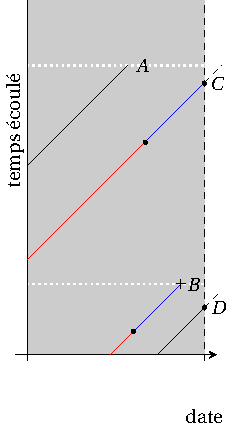
\includegraphics{figures/Lexis_censure_modif.pdf}
\end{column}

\begin{column}{0.6\textwidth}
Pour ajuster le modèle, on peut casser la contribution d'une observation
en segments: considérons un seul changement survenant au temps \(t_c\).

\begin{itemize}
\tightlist
\item
  pour le premier segment, on enregistre \(t_c\) comme valeur maximale
  (censure à droite)
\item
  pour la deuxième portion, l'observation est tronquée à gauche à partir
  de \(t_c\).
\end{itemize}
\end{column}
\end{columns}
\end{frame}

\begin{frame}[fragile]{Exemple}
\protect\hypertarget{exemple}{}
Supposons qu'il y a eu au plus un changement dans la variable
\texttt{service}. On doit formatter la base de données comme suit.

\footnotesize

\hypertarget{tbl-survie3-donnees}{}
\begin{table}
\caption{\label{tbl-survie3-donnees}Aperçu des cinq premières observations de la base de données survie3. }\tabularnewline

\centering
\begin{tabular}{rrrrrrll}
\toprule
id & debut & fin & evenement & age & sexe & region & service\\
\midrule
1 & 0 & 130 & 0 & 48 & 1 & 3 & 2\\
1 & 130 & 178 & 0 & 48 & 1 & 3 & 1\\
2 & 0 & 159 & 0 & 31 & 1 & 3 & 2\\
3 & 0 & 110 & 1 & 36 & 1 & 4 & 0\\
4 & 0 & 109 & 1 & 30 & 0 & 2 & 0\\
5 & 0 & 78 & 0 & 22 & 0 & 5 & 1\\
5 & 78 & 108 & 1 & 22 & 0 & 5 & 0\\
\bottomrule
\end{tabular}
\end{table}

Tout intervalle autre que terminal pour un individu est traité comme de
la censure à droite.

\normalsize
\end{frame}

\begin{frame}[fragile]{Code pour variables explicatives variables}
\protect\hypertarget{code-pour-variables-explicatives-variables}{}
\begin{Shaded}
\begin{Highlighting}[numbers=left,,]
\FunctionTok{data}\NormalTok{(survie3, }\AttributeTok{package =} \StringTok{"hecmulti"}\NormalTok{)}
\NormalTok{cox4 }\OtherTok{\textless{}{-}} \FunctionTok{coxph}\NormalTok{(}\FunctionTok{Surv}\NormalTok{(}\AttributeTok{time =}\NormalTok{ debut, }
                   \AttributeTok{time2 =}\NormalTok{ fin, }
                   \AttributeTok{event =}\NormalTok{ evenement) }\SpecialCharTok{\textasciitilde{}} 
\NormalTok{                age }\SpecialCharTok{+}\NormalTok{ sexe }\SpecialCharTok{+}\NormalTok{ service, }
              \AttributeTok{data =}\NormalTok{ survie3)}
\end{Highlighting}
\end{Shaded}

\footnotesize

Puisque c'est la valeur d'une variable qui varie dans le temps et non
pas son effet, on a l'interprétation usuelle.

\normalsize
\end{frame}

\begin{frame}{Modèle à risques compétitifs}
\protect\hypertarget{moduxe8le-uxe0-risques-compuxe9titifs}{}
Parfois, la raison pour laquelle un individu quitte l'état étudié peut
avoir un intérêt en soi.

Pour le temps de service d'un employé, on veut faire la distinction
entre

\begin{itemize}
\tightlist
\item
  une démission
\item
  un renvoi
\item
  la retraite
\end{itemize}
\end{frame}

\begin{frame}[fragile]{Exemple}
\protect\hypertarget{exemple-1}{}
Supposons que nous avons trois causes possibles pour la perte d'un
client. La variable \texttt{censure} dans le fichier \texttt{survie4}
vaut:

\begin{itemize}
\tightlist
\item
  \texttt{1} si l'individu est toujours abonné à notre service
\item
  \texttt{2} désabonnement pour aller chez le compétiteur A
\item
  \texttt{3} désabonnement pour aller chez le compétiteur B
\item
  \texttt{4} désabonnement parce qu'il n'a plus besoin de cellulaire.
\end{itemize}
\end{frame}

\begin{frame}{Transition d'un état à l'autre}
\protect\hypertarget{transition-dun-uxe9tat-uxe0-lautre}{}
\begin{columns}[T]
\begin{column}{0.6\textwidth}
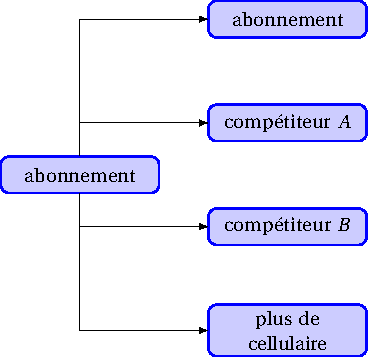
\includegraphics{figures/transition_etats_modele_risque_competitifs.pdf}
\end{column}

\begin{column}{0.4\textwidth}
Modèle avec transition d'un état de base (abonné) vers un état absorbant
(désabonnement, soit chez compétiteur \(A\), compétiteur \(B\) ou
abandon du cellulaire).
\end{column}
\end{columns}
\end{frame}

\begin{frame}{Modèle à risques compétitifs avec modèle de Cox}
\protect\hypertarget{moduxe8le-uxe0-risques-compuxe9titifs-avec-moduxe8le-de-cox}{}
Pour estimer la probabilité d'un événement au fil du temps, on peut
ajuster plusieurs modèles de Cox.

On spécifie une fonction de risque pour chaque événement compétitif,
\begin{align*}
h_1(t; \mathbf{X})&= h_{01}(t) \exp(\beta_{11}\mathrm{X}_1 + \cdots + \beta_{p1} \mathrm{X}_p),\\
&\vdots\\
h_K(t; \mathbf{X})&= h_{0K}(t) \exp(\beta_{1K}\mathrm{X}_1 + \cdots + \beta_{pK} \mathrm{X}_p).\\
\end{align*} Notez que les coefficients sont différents d'une équation à
l'autre.

On peut estimer les paramètres de chaque équation du modèle de Cox
séparément sans perte de précision en modifiant la définition de
l'événement.
\end{frame}

\begin{frame}[fragile]{Code \textbf{R} pour risque compétitif (1)}
\protect\hypertarget{code-r-pour-risque-compuxe9titif-1}{}
Deux options: ajuster chaque modèle séparément en traitant tout
événement autre que celui d'intérêt comme de la censure à droite.

\begin{Shaded}
\begin{Highlighting}[numbers=left,,]
\CommentTok{\# Rappel pour "event":}
\CommentTok{\#  {-} 1 (TRUE) pour observation, }
\CommentTok{\#  {-} 0 (FALSE) pour censure à droite}
\FunctionTok{data}\NormalTok{(survie4, }\AttributeTok{package =} \StringTok{"hecmulti"}\NormalTok{)}
\NormalTok{rc\_cox\_A }\OtherTok{\textless{}{-}} \FunctionTok{coxph}\NormalTok{(}\FunctionTok{Surv}\NormalTok{(}\AttributeTok{time =}\NormalTok{ temps, }
                   \AttributeTok{event =}\NormalTok{ censure }\SpecialCharTok{==} \DecValTok{2}\NormalTok{) }\SpecialCharTok{\textasciitilde{}} 
\NormalTok{                age }\SpecialCharTok{+}\NormalTok{ sexe }\SpecialCharTok{+}\NormalTok{ service, }
              \AttributeTok{data =}\NormalTok{ survie4)}
\end{Highlighting}
\end{Shaded}

\footnotesize

Les observations avec des valeurs pour \texttt{censure} de 1, 3 ou 4
sont traitées comme des cas de censure à droite (l'événement quitter
pour compétiteur \(A\) n'est pas survenu).

\normalsize
\end{frame}

\begin{frame}{Interprétation des coefficients}
\protect\hypertarget{interpruxe9tation-des-coefficients}{}
Attention, l'interprétation dépend maintenant de l'événement étudié.

\begin{table}
\centering
\begin{tabular}{lrrr}
\toprule
terme & exp(coef) & borne inf. & borne sup.\\
\midrule
age & 0.96 & 0.94 & 0.974\\
sexe & 0.48 & 0.35 & 0.673\\
service1 & 0.38 & 0.27 & 0.535\\
service2 & 0.19 & 0.11 & 0.308\\
service3 & 0.11 & 0.05 & 0.220\\
\bottomrule
\end{tabular}
\end{table}

Selon le modèle, le risque \emph{de quitter pour aller chez le
compétiteur A} d'une femme est 0.48 fois celui d'un homme.
\end{frame}

\begin{frame}[fragile]{Code \textbf{R} pour risque compétitif (2)}
\protect\hypertarget{code-r-pour-risque-compuxe9titif-2}{}
Créer une variable avec identifiant \(1, \ldots, n\).

Passer la variable état comme \textbf{facteur}, avec transition depuis
catégorie de référence (ici \texttt{censure=1}, soit abonné)

\begin{Shaded}
\begin{Highlighting}[numbers=left,,]
\NormalTok{n }\OtherTok{\textless{}{-}} \FunctionTok{nrow}\NormalTok{(survie4)}
\NormalTok{surv4 }\OtherTok{\textless{}{-}}\NormalTok{ survie4 }\SpecialCharTok{|\textgreater{}} 
\NormalTok{  dplyr}\SpecialCharTok{::}\FunctionTok{mutate}\NormalTok{(}\AttributeTok{id =} \FunctionTok{seq\_len}\NormalTok{(n))}
\NormalTok{rc\_cox }\OtherTok{\textless{}{-}} \FunctionTok{coxph}\NormalTok{(}\FunctionTok{Surv}\NormalTok{(}\AttributeTok{time =}\NormalTok{ temps, }
             \AttributeTok{event =} \FunctionTok{factor}\NormalTok{(censure)) }\SpecialCharTok{\textasciitilde{}} 
\NormalTok{               sexe }\SpecialCharTok{+}\NormalTok{ age }\SpecialCharTok{+}\NormalTok{ service,}
             \AttributeTok{data =}\NormalTok{ surv4,}
             \AttributeTok{id =}\NormalTok{ id)}
\end{Highlighting}
\end{Shaded}

\footnotesize

L'identifiant sert dans les cas où on peut transiter entre plusieurs
états et il y a plusieurs observations pour un même individu.
\end{frame}

\begin{frame}[fragile]{Code \textbf{R} pour risques compétitifs
(Kaplan--Meier)}
\protect\hypertarget{code-r-pour-risques-compuxe9titifs-kaplanmeier}{}
Ajuster le modèle multi-état avec un \textbf{facteur} pour l'événement,
où la catégorie de référence est abonnement (\texttt{censure=1}).

Surtout, ne pas estimer les courbes séparément!

\begin{Shaded}
\begin{Highlighting}[numbers=left,,]
\FunctionTok{data}\NormalTok{(survie4, }\AttributeTok{package =} \StringTok{"hecmulti"}\NormalTok{)}
\NormalTok{rc\_km }\OtherTok{\textless{}{-}} \FunctionTok{survfit}\NormalTok{(}\FunctionTok{Surv}\NormalTok{(}\AttributeTok{time =}\NormalTok{ temps, }
             \AttributeTok{event =} \FunctionTok{factor}\NormalTok{(censure)) }\SpecialCharTok{\textasciitilde{}} \DecValTok{1}\NormalTok{, }\CommentTok{\#facteur}
             \AttributeTok{data =}\NormalTok{ survie4)}
\end{Highlighting}
\end{Shaded}
\end{frame}

\begin{frame}{Graphiques}
\protect\hypertarget{graphiques}{}
Les représentations graphiques donnent la probabilité d'être dans une
situation en fonction du temps (ici avec la catégorie de référence
abonnement).

\footnotesize

\begin{figure}

{\centering \includegraphics[width=1\textwidth,height=\textheight]{MATH60602-diapos9_files/figure-beamer/fig-competitif-1.pdf}

}

\caption{\label{fig-competitif}Probabilité d'événement sans variable
explicative (Kaplan-Meier, gauche) et avec âge, service et sexe (modèle
de Cox, droite).}

\end{figure}
\end{frame}

\begin{frame}{Récapitulatif}
\protect\hypertarget{ruxe9capitulatif}{}
Si le postulat de risques proportionnels ne tient pas, on peut
considérer des modifications du modèle de Cox.

\begin{itemize}
\tightlist
\item
  stratification (uniquement pour variables catégorielles) pour estimer
  le risque de base séparément sur chaque sous-groupe).
\item
  modèle à risques non-proportionnels avec variable ou coefficient qui
  varient selon le temps
\end{itemize}
\end{frame}

\begin{frame}{Récapitulatif}
\protect\hypertarget{ruxe9capitulatif-1}{}
Si les variables explicatives changent au fil du temps, on peut traiter
le cas de figure en décomposant la contribution de l'observation en
plusieurs segments

\begin{itemize}
\tightlist
\item
  chaque segment autre que terminal est traité comme de la censure à
  droite
\item
  les segments sont sujets à troncature à gauche.
\end{itemize}

La base de données doit contenir le temps initial et le temps final de
l'intervalle, en plus de l'indicateur.

Il y a un lien possible avec le modèle à risque proportionnels si
l'effet est le même pour tous (comme l'âge).
\end{frame}

\begin{frame}{Récapitulatif}
\protect\hypertarget{ruxe9capitulatif-2}{}
Le modèle multi-état (modèle à risques compétitifs) permet d'estimer la
probabilité de chaque transition.

\begin{itemize}
\tightlist
\item
  la survie pour l'événement de base reste le même (désabonnement)
\item
  à chaque temps donné, la probabilité conjointe de chaque \(K+1\)
  possibilités est 1.
\end{itemize}

Dans \textbf{R}, s'assurer que la catégorie de référence est l'état de
départ.
\end{frame}



\end{document}
